\documentclass{beamer}
\usetheme{Metropolis}
%\usebeamercolor{lily}
\useoutertheme{infolines}
\usefonttheme{serif}
\usepackage{graphicx}
\usepackage{setspace}
\usepackage{tabularx}
\usepackage{tikzsymbols}
\usepackage{tikz}
\usepackage{spot}
\usepackage[italian]{babel}
\usepackage{tabularx}
\usepackage[absolute,overlay]{textpos}
\usepackage{booktabs}



\newcommand\Factor{1.2}



\setbeamerfont{subtitle}{size=\large, series=\bfseries}
\definecolor{template}{RGB}{54, 114, 89}
\definecolor{background}{RGB}{250, 250, 250}
\setbeamercolor{frametitle}{fg=template, bg=background}
\setbeamercolor{section in head/foot}{bg=template}
\setbeamercolor{subsection in head/foot}{bg=template!20, fg=template}
\setbeamercolor{author in head/foot}{bg=template}
\setbeamercolor{date in head/foot}{bg=template}
\setbeamercolor{title in head/foot}{fg=template}
\setbeamertemplate{frametitle}[default][center]
\setbeamercolor{title}{fg=template}
\definecolor{back}{RGB}{247, 251, 255}
\definecolor{map}{RGB}{111, 172, 232}
\definecolor{childmap}{RGB}{161, 200, 240}
\definecolor{nodemap}{RGB}{141, 170, 199}
\definecolor{rasch}{rgb}{0.0, 0.33, 0.71}
\definecolor{log}{rgb}{0.0, 0.65, 0.58}
\definecolor{diff}{RGB}{33, 113, 181}
\definecolor{single}{RGB}{106, 81, 163}
\definecolor{comp}{RGB}{35, 99, 70}
\definecolor{inc}{RGB}{191, 13, 43}
\definecolor{highlight}{rgb}{0.45, 0.31, 0.59}
\definecolor{section}{RGB}{51,51,179}
\definecolor{typical}{RGB}{8, 69, 148}
\definecolor{model}{RGB}{74, 20, 134}
\definecolor{orangered2}{RGB}{238,64,0}
\definecolor{royalblue3}{RGB}{58,95,205}
\definecolor{springgreen}{RGB}{0,205,102}
\definecolor{magenta}{RGB}{255,0,255}

  \tikzset{
	invisible/.style={opacity=0},
	visible on/.style={alt={#1{}{invisible}}},
	alt/.code args={<#1>#2#3}{%
		\alt<#1>{\pgfkeysalso{#2}}{\pgfkeysalso{#3}} % \pgfkeysalso doesn't change the path
	},
	every overlay node/.style={
		%draw=black,fill=white,rounded corners,
		anchor=north west, inner sep=0pt,
	},
}

\def\tikzoverlay{%
	\tikz[remember picture, overlay]\node[every overlay node]
}%

\AtBeginSection[]
{
	\begin{frame}
		\frametitle{Table of Contents}
		\tableofcontents[currentsection]
	\end{frame}
}  


%\title[Implicit assessment]{Implicit assessment in psychology: \\ How to work with the IAT}
\title[Experiment set up]{Misurazione Implicita in Psicologia: \\ Impostare gli esperimenti}
\date[PSQT]{Master di II secondo Livello in \\ Psicologia quantitativa. Misurazione, valutazione e analisi di variabili psicosociali }
\institute[]{22 luglio 2022, Padova}
\author[Ottavia Epifania]{\texorpdfstring{Dr. Ottavia M. Epifania\newline\url{ottavia.epifania@unipd.it}}{Author}}

\begin{document}
	\tikzstyle{every picture}+=[remember picture]
	
	


\begin{frame}[plain]
    \maketitle
\end{frame}

\begin{frame}{Contenuti}
	\tableofcontents
\end{frame}

\section{Cosa ci serve}

\begin{frame}
	
	\begin{itemize}
			\item Download \href{https://www.millisecond.com/download/}{
\includegraphics[width=0.10\linewidth]{inquisit.png}} e seguire le istruzioni \textcolor{red}{!!! la demo è valida solo per un mese!!}
			\item Download the \href{https://www.millisecond.com/download/library/iat/ageiat}{\textcolor{blue}{AGE IAT}} from Inquisit test library
		\item \href{https://www.millisecond.com/download/library}{\textcolor{blue}{The Inquisit Test library}} 
	\end{itemize}
\end{frame}

\begin{frame}
	Open the file and run the experiment! 
	
	Once you're done, send me the resulting \texttt{.dat} file (we'll use this afternoon for the data analysis part)
	
	Did you like the experiment? Would you change something? Would you add something? 
\end{frame}

\section{The Inquisit file}
\begin{frame}
	\begin{enumerate}
		\item User manual (keep it or not)
		\item Welcome 
		\item Etichette e stimoli
		\item Pagine di istruzione \& summary dei risultati
		\item Preparare il materiale
		\item Preparare i ``blocchi'' dell'esperimento
		\item L'esperimento
	\end{enumerate}
\end{frame}

\subsection*{Welcome}

\begin{frame}[fragile]
	
	\begin{columns}
	\begin{column}{.50\linewidth}
		\begin{small}
				\begin{verbatim}
				<htmlpage iatintro>
				/ file = "intro_pictureiat.htm"
				</htmlpage>
			\end{verbatim}
		\end{small}
	\end{column}

	\begin{column}{.50\linewidth}
		\centering
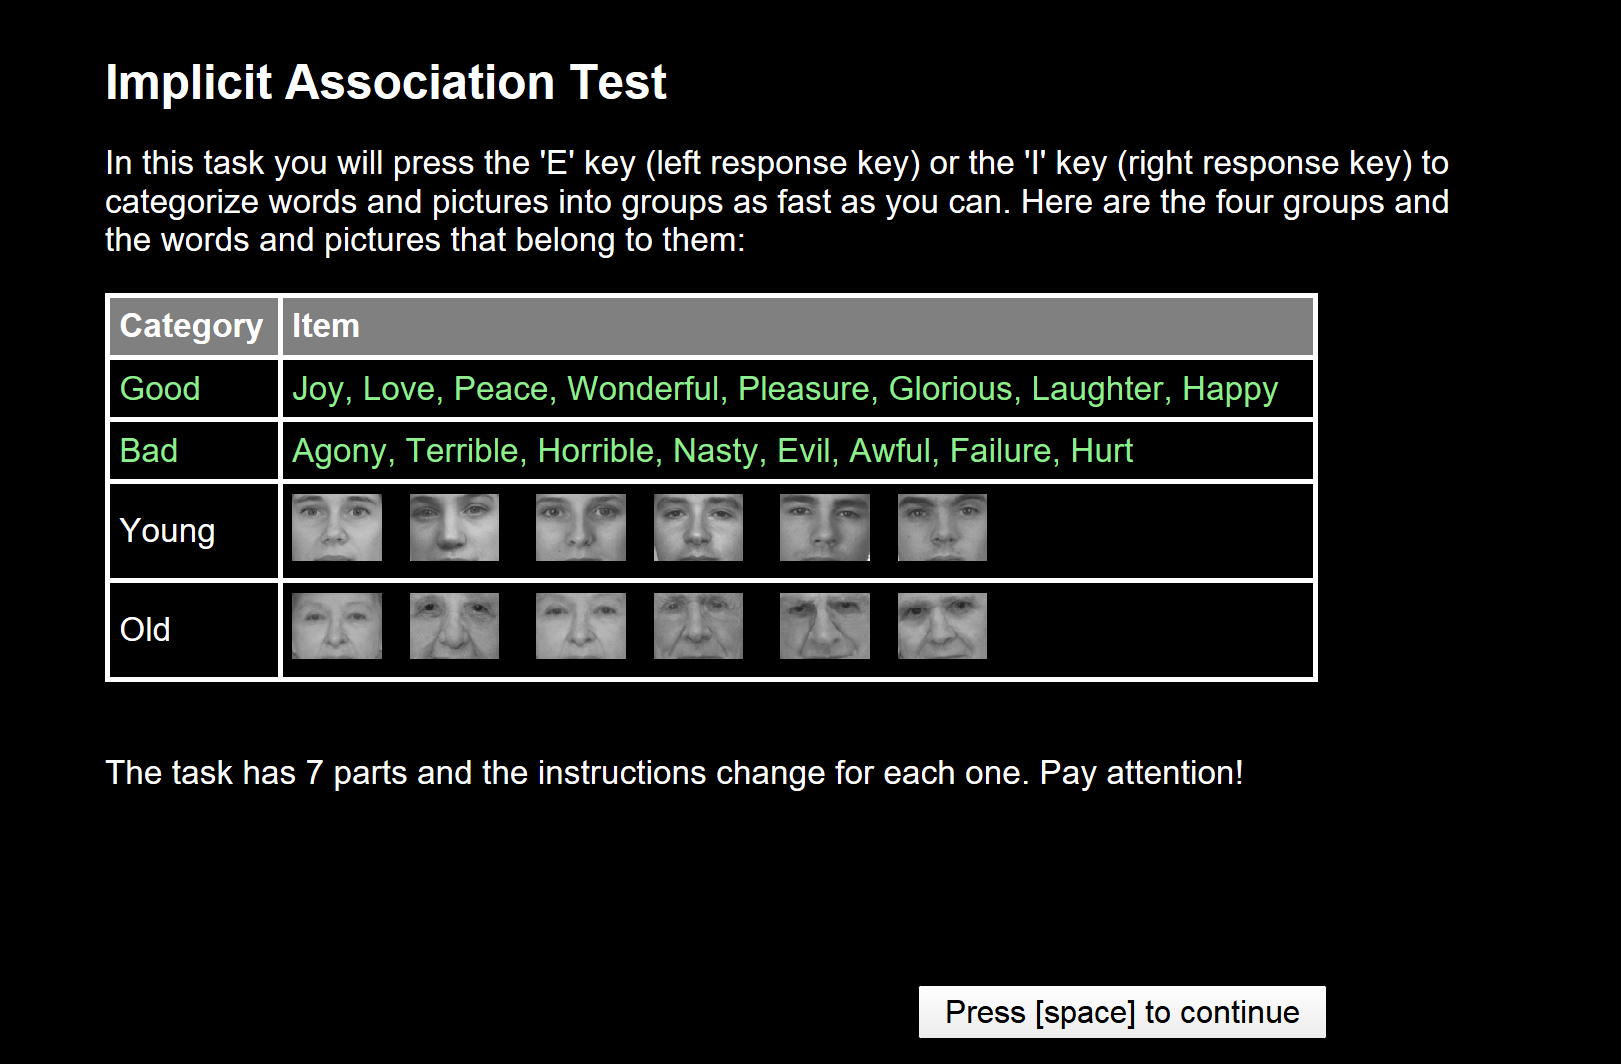
\includegraphics[width=\linewidth]{iatIntro.png}
   \end{column}
	\end{columns}
	
\end{frame}

\begin{frame}[fragile]
	 \texttt{intro\_pictureiat.htm} Si apre con il blocco note 
	
\begin{footnotesize}
		\begin{verbatim}
		<!DOCTYPE html>
		<html>
		<head>
		<meta charset="UTF-8">
		<meta name="robots" content="noindex, nofollow"/> 
		<title>iat intro</title>
		<style>
		.center {
			text-align: center;
		}
		.left {	
			text-align: left;
		}
		[.....]
	\end{verbatim}
\end{footnotesize}

Può essere modificato e salvato (ad esempio, per mettere le istruzioni in italiano)
\end{frame}

\subsection*{Etichette e stimoli}

\begin{frame}[fragile]
	Define ``Attribute A'' (in this case, ``\textcolor{green}{Good}'')
	
	\begin{columns}
		\begin{column}[T]{.50\linewidth}
			\begin{small}
					\begin{verbatim}
					<item attributeAlabel>
					/1 = "Good"
					</item>
					
					<item attributeA>
					/1 = "Joy"
					/2 = "Love"
					/3 = "Peace"
					/4 = "Wonderful"
					/5 = "Pleasure"
					/6 = "Glorious"
					/7 = "Laughter"
					/8 = "Happy"
					</item>
				\end{verbatim}
			\end{small}
		\end{column}
	
		\begin{column}[T]{.50\linewidth}
			\vspace{5mm}
		Definisce la prima delle dimensioni valutative (i.e., ``Good'')
		
		\vspace{10mm}
		
		Elenco di tutte le parole che appartengono a ``Good''
		
		Per aggiungere ulteriori parole: \\ \texttt{/9 = ``Bello''  \\  /10 = ``Carino''}
	\end{column}
	\end{columns}



\end{frame}

\begin{frame}[fragile]
	Same thing with the target category ``Target A'' (`in this case ``Young'' ), just remember to import the images (have to be in the same folder)
	
	\begin{columns}
		\begin{column}[T]{.50\linewidth}
			\begin{small}
			\begin{verbatim}
				<item targetAlabel>
				/1 = "Young"
				</item>
				
				<item targetA>
				/1 = "yf1.jpg"
				/2 = "yf4.jpg"
				/3 = "yf5.jpg"
				/4 = "ym2.jpg"
				/5 = "ym3.jpg"
				/6 = "ym5.jpg"
				</item>
			\end{verbatim}
			\end{small}
		\end{column}
		
		\begin{column}[T]{.50\linewidth}
			\vspace{5mm}
			First define the label of the target category (i.e., ``Young'')
			
			\vspace{10mm}
			
			List all the elements belonging to the superordinate category ``Young'' (i.e., the images in the same folder)
		\end{column}
	\end{columns}
	
\end{frame}

\subsection*{Instruction pages \& Performance summary}

\begin{frame}[fragile]
		\begin{verbatim}
			<instruct>
			/ navigationbuttonfontstyle = 
			("Arial", 3%, false, false, false, false, 5, 1)
			</instruct>
		\end{verbatim}
	
	This defines the button to navigate through pages. Here you define its appearance, not its behavior. 
	
	To change the font:
	
	\begin{verbatim}
		("font-name", height, bold, italic, underline, strikeout, 
		quality, set)
	\end{verbatim}

font-name: e.g., ``Arial'', ``Tahoma'', ``Courier New''

quality: quality of the font, 1-5

set: characters set (e.g., latin, greek. 1 stands for the default of the computer on which Inquisit runs)
	\end{frame}

\begin{frame}[fragile]
	
	\begin{verbatim}
		
	<item instructions>
	/ 1 = "Put your left[...]."
	
	/ 2 = "Put your left finger [...]"
	
	/ 3 = "Press the left 'E' "
	
	[...]
	</item>
\end{verbatim}

\vspace{5mm}
Same as the attribute stimuli ``Good'', here the instructions are defined as a list of items

Again, this is only the content of the instructions

\end{frame}

\begin{frame}[fragile]
	\begin{verbatim}
		'<%item.attributeAlabel.item(1)%>' 
	\end{verbatim}

Allows for automatically including the label of attribute A in the instruction text. It uses ``item'' because it is supposed to be ``fixed''

\begin{verbatim}
	'<%expressions.leftTarget%>'
\end{verbatim}

Allows for automatically including the target \textbf{displayed on the left side of the screen}. It uses ``expressions'' because the target displayed on the left side of the screen changes according to the experiment 

\end{frame}


\begin{frame}[fragile]
\begin{figure}
	\centering
	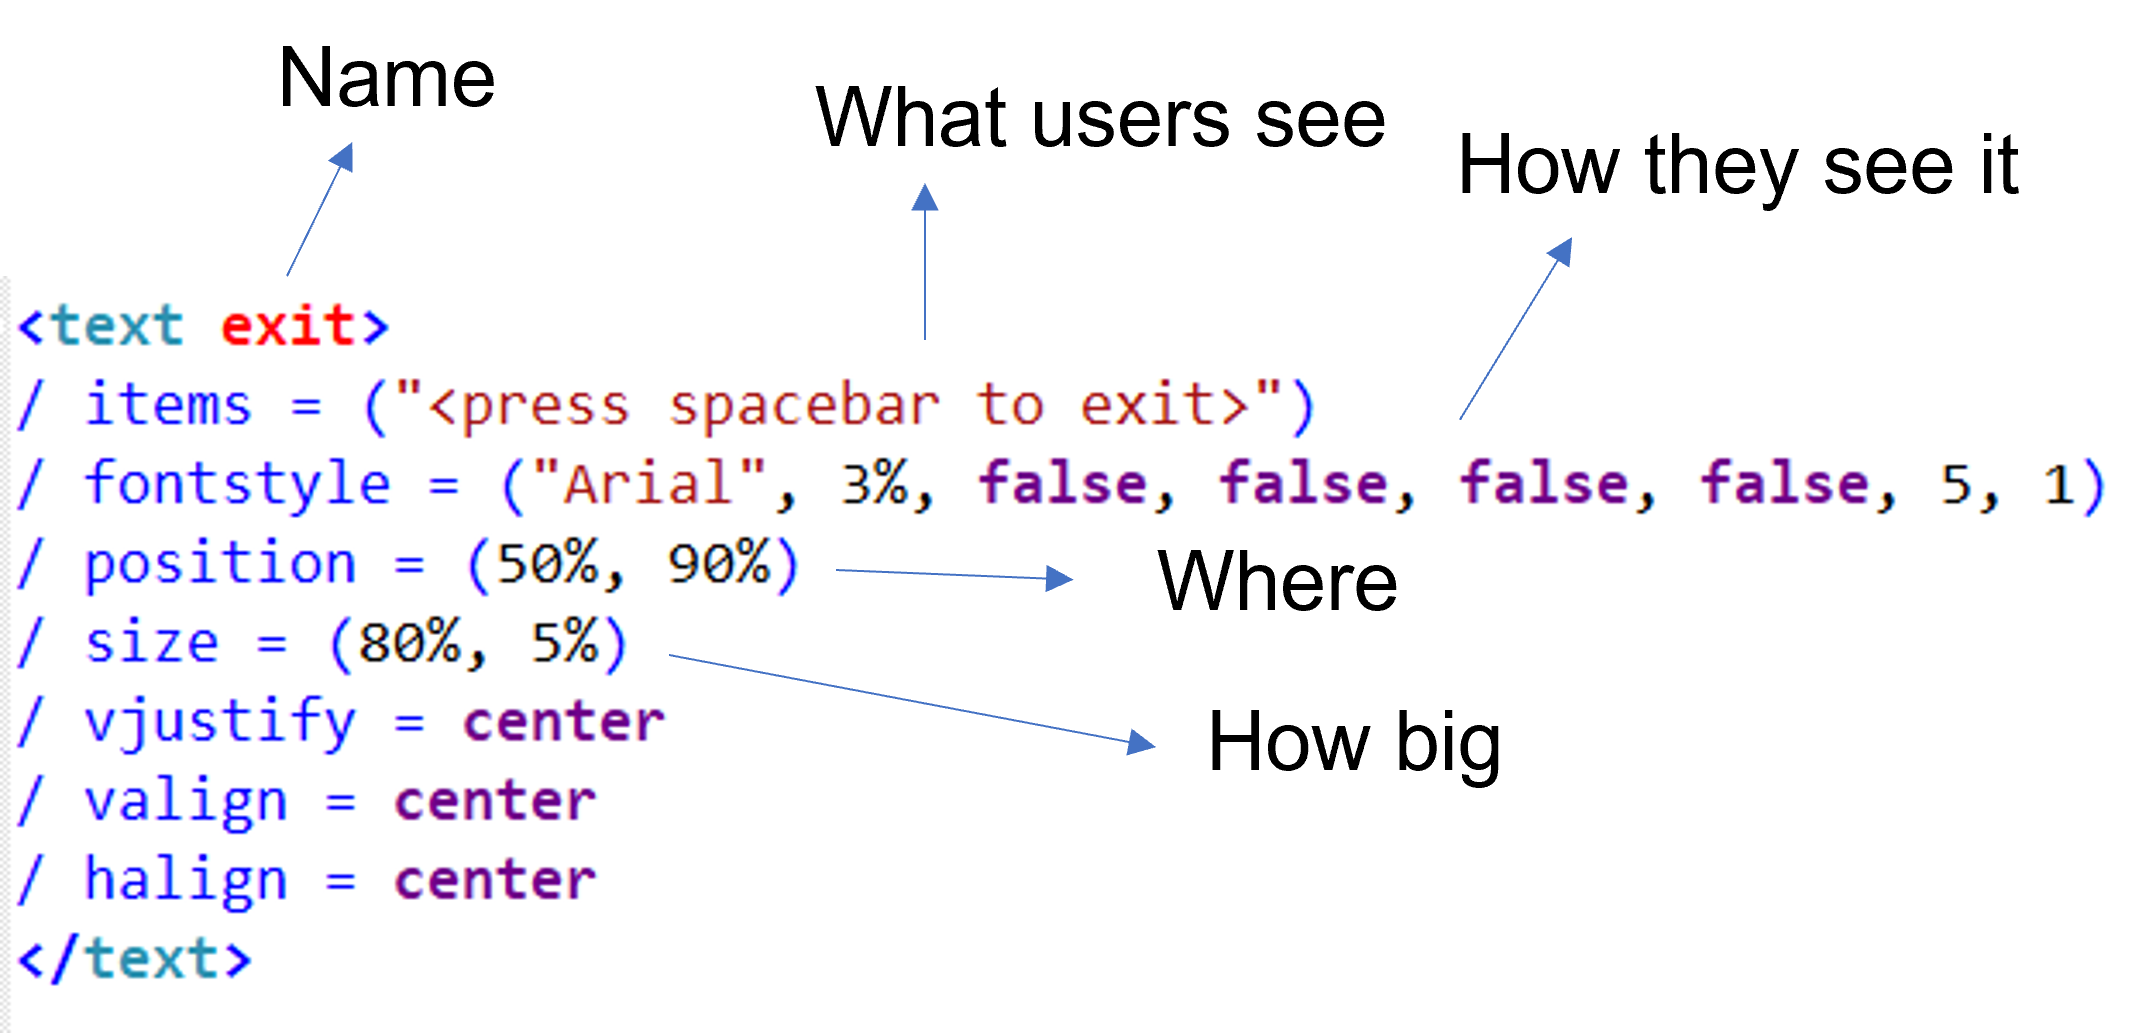
\includegraphics[width=.80\linewidth]{textThank.png}
\end{figure}

\vspace{3mm}
No actual behavior has been defined yet
\end{frame}

\subsection*{Set up the experiment material}
\begin{frame}[fragile]
	Use what defined in \texttt{<item instructions>} (\texttt{/items = instructions}) and add some fancy formatting: 
	
	\begin{verbatim}
		<text instructions>
		/ items = instructions
		/ position = (10%, 25%)
		/ halign = left
		/ valign = top
		/ hjustify = left
		/ vjustify = center
		/ size = (80%, 50%)
		/ select = values.instructionIndex
		</text>
	\end{verbatim}

\texttt{/ select = values.instructionIndex} tells which page of instructions to show

\end{frame}

\begin{frame}[fragile]
	\begin{small}
		With \texttt{<trial instructions>} we finally set the behavior of  ``instructions'' throughout the experiment: 
	
	\begin{verbatim}
		<trial instructions>
		/ ontrialbegin = [
		values.progresswidth += 10;
		values.instructionIndex += 1;
		]
		/ stimulustimes = [1=instructions, spacebar, progressbar, progressbar_fill]
		/ correctresponse = (" ")
		/ errormessage = false
		/ recorddata = false
		/ showmousecursor = true
		</trial>
	\end{verbatim}
	
	\texttt{/ stimulustimes = [1=instructions, spacebar, progressbar, progressbar\_fill]} $\rightarrow$ stimuli that have to be included in the \texttt{instructions} trial.
	\end{small}


\end{frame}

\begin{frame}[fragile]
	Set the appearance of the word stimuli: 
	\vspace{3mm}
	\begin{verbatim}
		<text attributeA>
		/ items = attributeA
		/ fontstyle = ("Arial", 5%)
		/ txcolor = green
		</text>
	\end{verbatim}
\vspace{3mm}

Set the behavior of the stimuli!
\begin{verbatim}
	<trial attributeA>
	/ validresponse = ("E", "I")
	/ correctresponse = ("E")
	/ stimulusframes = [1 = attributeA, errorReminder]
	/ posttrialpause = parameters.ISI
	</trial>
\end{verbatim}

\end{frame}

\begin{frame}[fragile]
	Set the appearance of the stimuli: 
	\vspace{3mm}
	\begin{verbatim}
<picture targetA>
/ items = targetA
/ size = (20%, 20%)
</picture>
	\end{verbatim}
	\vspace{3mm}
	
	Set the behavior of the stimuli.
	\begin{verbatim}
<trial targetAleft>
/ validresponse = ("E", "I")
/ correctresponse = ("E")
/ stimulusframes = [1 = targetA, errorReminder]
/ posttrialpause = parameters.ISI
</trial>
	\end{verbatim}
	
\end{frame}

\subsection*{Set up the experiment blocks}

\begin{frame}
	\begin{figure}
		\centering
		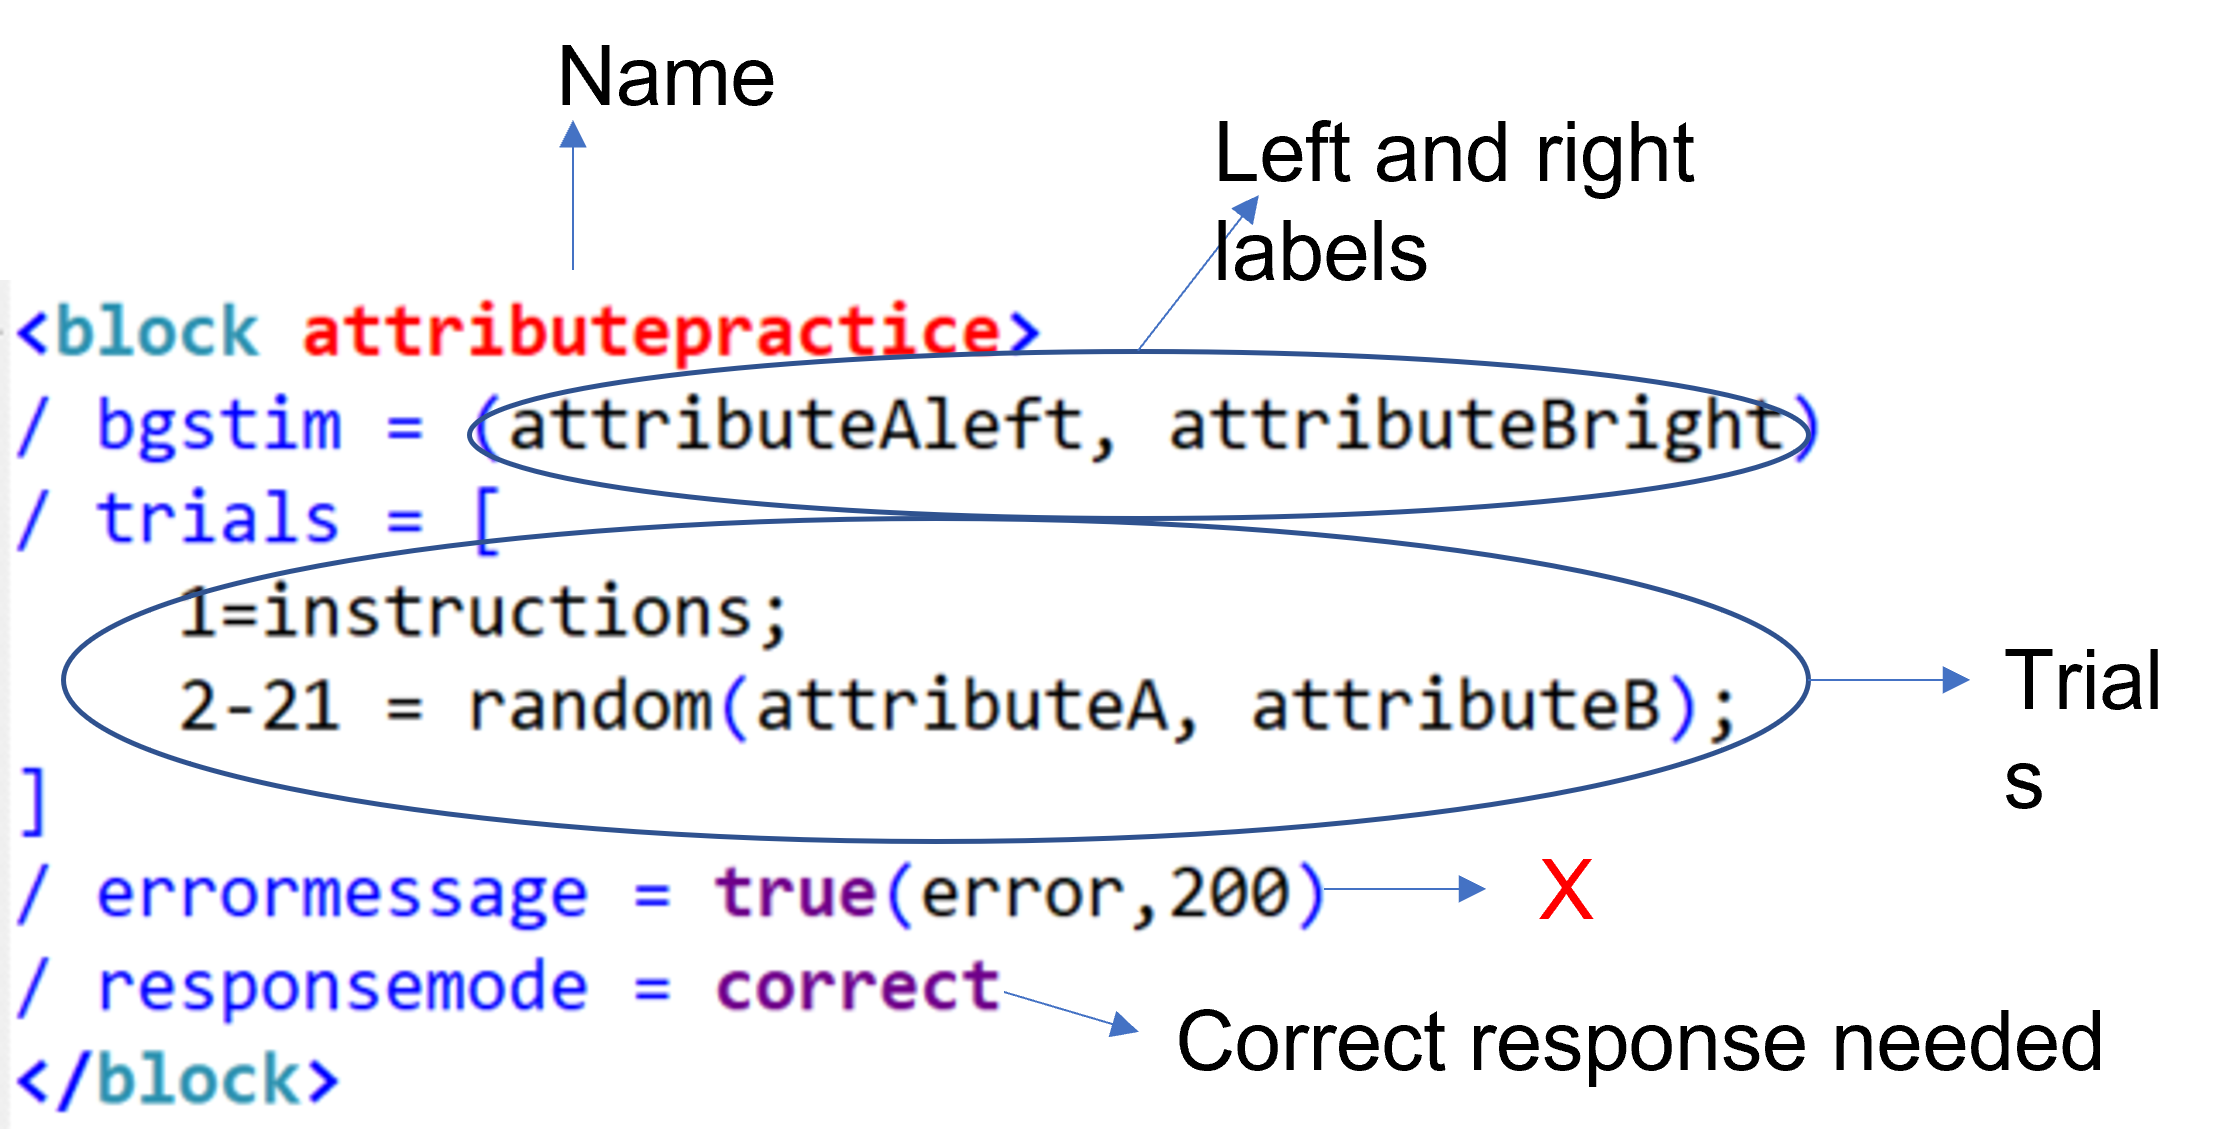
\includegraphics[width=.80\linewidth]{block.png}
	\end{figure}
\vspace{3mm}
\texttt{1=instructions;} First trial is an instruction page (the first one)

\texttt{2-21 = random(attributeA, attributeB);} Trials from 2 to 21 are randomly drawn from \texttt{attributeA} and \texttt{attributeB} stimuli

Total number of trials = 20
\end{frame}


\begin{frame}[fragile]
\begin{verbatim}
	/ bgstim = (targetAleftmixed, orleft, attributeAleft, targetBrightmixed, orright, attributeBright)
	/ trials = [
	1=instructions;
	3,5,7,9,11,13,15,17,19,21= random(targetAleft, targetBright);
	2,4,6,8,10,12,14,16,18,20 = random(attributeA, attributeB)]
	/ errormessage = true(error,200)
	/ responsemode = correct
	[...]
\end{verbatim}

Target and stimuli are presented one at a time, one image, one word
\end{frame}

\section{Experiment time!}


\begin{frame}[fragile]{Primo gruppo}
	\begin{small}
			\begin{verbatim}
			<expt>
			/ onexptbegin = [
			values.conditionOrder = "c-ic" % associative conditions order
			]
			/ preinstructions = (iatintro) % the ``welcome'' page
			/ groups = (1 of 2) % actual conditions presentation
			/ blocks = [   % the IAT itself
         	1=targetcompatiblepractice; 2=attributepractice; 
            3=compatibletest1; 	4=compatibletestinstructions;	5=compatibletest2; 
            6=targetincompatiblepractice; 7=incompatibletest1; 
            8=incompatibletestinstructions;	9=incompatibletest2; 
            10=summary;  % the results
            11 = end; % goodbye
			]
			</expt>
		\end{verbatim}
	\end{small}
\end{frame}


\begin{frame}[fragile]{Secondo gruppo}
	\begin{small}
		\begin{verbatim}
			<expt>
			/ onexptbegin = [
			values.conditionOrder = "ic-c"
			]
			/ preinstructions = (iatintro)
			/ groups = (2 of 2) % change the grouping
			/ blocks = [ % change the conditions presentation order
			1=targetincompatiblepractice; 	2=attributepractice; 
			3=incompatibletest1; 4=incompatibletestinstructions; 5=incompatibletest2; 
			6=targetcompatiblepractice; 7=compatibletest1; 
			8=compatibletestinstructions; 9=compatibletest2; 
			10=summary;
			11 = end;
			]
			</expt>
		\end{verbatim}
	\end{small}
\end{frame}

\begin{frame}
	Si possono avere tutti i gruppi che si vogliono, a seconda del numero di condizioni sperimentali 
	
	In questo caso: 
	
	\begin{itemize}
		\item Tutti i soggetti dispari \texttt{/ groups = (1 of 2)} vedono prima la condizione compatibile e poi quella incompatibile
			\item Tutti i soggetti pari \texttt{/ groups = (2 of 2)} vedono prima la condizione incompatibile e poi quella compatibile
	\end{itemize}

Se avessimo un questionario, dovremmo specificarlo qui nell'ordine in cui vogliamo presentarlo rispetto alle misure implicite
\end{frame}

\section*{Tempo di modifiche}

\begin{frame}
	La prima cosa da fare, ovviamente, è tradurre il tutto in italiano (vi lascio divertire)
	
	Attenzione! Per non complicare troppo le operazioni, si possono tradurre solo le parti che i partecipanti vedranno
	 
\end{frame}

\end{document}